% =====================================================================
%  Chapter 4 — The Replication Crises, and What to Do About Them
% =====================================================================

\chapter{The Replication Crises, and What to Do About Them}
\label{ch:replication-crisis}

Chapter 3 surveyed what the evidence says. This chapter asks a different
question: given that evidence, what would a professional research process
have to do differently in order to find something, and can one person do
it?

\section{The machinery of self-deception}

There is a specific and well-documented failure mode in empirical finance,
and it is worth naming precisely because everything in Parts IV and VI is
built to detect it.

The procedure looks like this. A researcher has a dataset. They form a
hypothesis --- often a plausible economic story about why a variable should
predict returns. They test it. It does not work. They try variations: a
different formation window, a different weighting, a different sample
period, a different definition of the variable, dropping outliers, adding
an interaction. Eventually one of them works. The researcher writes the
paper about the one that worked.

Nothing in that story is dishonest. Every step is legitimate. And the
aggregate result is a literature in which the median published result is
smaller than the noise, in which the standard errors are too small, in
which a third of the results no longer work in their own original sample,
and in which the professional industry, applying the same methods at scale
and with far more resources, loses to a passive index on every long window
measured.

The failure is not in any individual step. It is in the fact that the
\emph{record of the steps} is not kept.

\section{What the selection bias is worth, quantitatively}

The magnitude of this bias is computable, and the book computes it.

If a researcher tries \(N\) variants of a strategy and reports the best
one, the expected best Sharpe ratio is not the Sharpe ratio of the
population of strategies; it is the maximum of a sample. The excess is
governed by the \emph{variance of the Sharpe ratio across trials} and by
the number of trials.

For a portfolio strategy with \(T\) months of returns, the estimated
Sharpe ratio has a standard error of approximately
\begin{equation}
\mathrm{SE}(\hat{SR}) \approx \frac{1}{\sqrt{T - 1}},
\end{equation}
in the i.i.d.\ case, and Lo's 2002 correction replaces this with a
scale factor \(\eta(T)\) that accounts for the serial correlation in the
returns --- the loss from serially correlated returns is large, because the
effective number of independent observations is much smaller than \(T\).

The expected maximum of \(N\) draws from a normal distribution with mean
\(\mu\) and standard deviation \(\sigma\) is
\begin{equation}
E\!\left[\max_{i \le N} Z_i\right] \approx
\frac{(1-\gamma)\,\Phi^{-1}\!\left(1 - \frac{1}{N}\right)
      + \gamma\,\Phi^{-1}\!\left(1 - \frac{1}{Ne}\right)}{},
\end{equation}
in the form that the Deflated Sharpe Ratio uses, and the whole point of the
Deflated Sharpe Ratio is to compare an observed Sharpe against
\emph{that} threshold rather than against zero.

Put plainly: if you tried one hundred strategies and the true Sharpe of
every one of them was zero, the best of the hundred would show a Sharpe of
roughly 0.8 to 1.0 in a 26-year sample. It would look like a triumph. It
would be arithmetic.

This is why the book reports, for every headline claim, the number of
strategies that were tried to produce it. Not as a methodological footnote
--- as a headline. Chapter 22 gives the machinery; Chapter 33 runs it on
this system's own family of \numFamilySize{} variants.

\begin{figure}[!htbp]
\centering
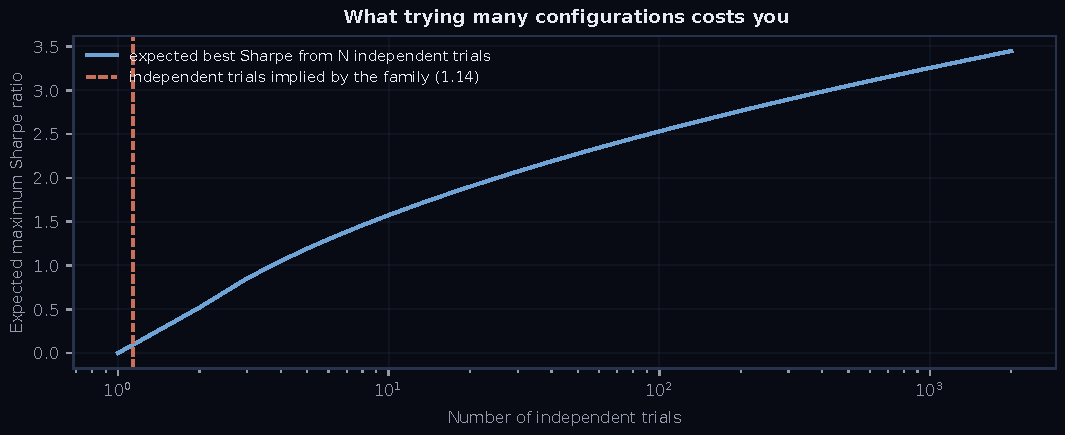
\includegraphics[width=\textwidth]{../figures/fig_deflated.pdf}
\caption{The Deflated Sharpe Ratio construction. The left panel shows the
distribution of the Sharpe ratio across the trial family and the
expected maximum of that distribution under the null; the right panel shows
the probability that the observed Sharpe exceeds the threshold, as a
function of the number of trials tried.}
\label{fig:deflated}
\end{figure}

\section{The second, subtler bias: trials are not independent}

There is a further difficulty that the Deflated Sharpe Ratio handles only
partially, and that this book handles explicitly.

Most of the variants a researcher tries are not independent of one another.
A momentum signal at a twelve-month horizon and at a thirteen-month horizon
are nearly the same strategy; the change in Kelly fraction from 0.10 to
0.50 is a rescaling of the same positions; and the members of this book's
model ensemble differ from each other only in which features they use and
which prior they carry.

If the trials are correlated, then trying more of them buys less
information about the maximum. The correct number of trials is therefore
not the number of configurations run but the number of
\emph{effectively independent} ones, and the two differ by a large factor.
This book computes the implied number of independent trials directly from
the correlation matrix of the trial family:
\begin{equation}
N^{*} = \hat{\rho} + (1 - \hat{\rho})\,M,
\end{equation}
where \(M\) is the raw number of trials and \(\hat{\rho}\) is the average
pairwise correlation of their returns, computed as
\begin{equation}
\hat{\rho} = \frac{\sum_{i}\sum_{j}\rho_{ij} - M}{M(M-1)}.
\end{equation}
The quantity \(N^{*}\) replaces \(M\) in the Deflated Sharpe Ratio. When
the members of a family produce nearly identical portfolios --- which they
do, in this book, for reasons the book examines --- \(N^{*}\) collapses
towards one, and the deflation is correspondingly weaker. That is correct
behaviour: a family of strategies that all do the same thing really is
approximately one trial.

\section{The third bias: the test is chosen after the data}

There is a selection effect even in the choice of the \emph{test}. If a
researcher computes a \(t\)-statistic for a hundred variants and reports the
one with the largest \(t\), the reported \(t\) is biased upwards in a way
that no correction to the standard error can undo. This is why the
literature has produced tests specifically designed for it: the White
reality check, which asks whether the \emph{best} of a family beats a
benchmark better than the family would by chance, and Hansen's test for
superior predictive ability, which asks the same question while accounting
for the fact that the family members are not equally good and should not be
weighted equally.

Both are implemented in this book, from their definitions rather than from
a library, and both are applied to the system's own family rather than to a
family chosen by someone else. Chapter 22 derives them; Chapter 33 reports
what they say.

\section{The fourth bias: the benchmark is not what you think}

A subtlety that catches even careful researchers. The comparison that
matters is not against a passive index that was chosen after the fact, and
not against a zero return. It is against the \emph{best strategy the investor
could have run instead}, which includes doing nothing, and includes the
strategy that a sensible person would have run with the same information.

This is why the trial family in this book is deliberately wide. It contains
the model configurations, the ablations that turn each layer off, the
sizing variants, and the alternative strategic policies. A reality check
over near-identical configurations would pass trivially and would mean
nothing. The check is only informative when the family contains the
alternatives a rational investor would actually have considered --- and the
ablation that says ``turn the machine off'' is the most important member
of that family, because it is the alternative a rational investor would
have considered first.

\begin{takeaway}[The protocol this book commits to]
\begin{enumerate}
\item Every configuration tried is written down before the test is run, and
the count is published.
\item The trial family includes the ablations, the sizing variants and the
alternative policies --- not only the configurations that might work.
\item The number of \emph{effectively independent} trials is computed from
the family's own correlation matrix, and used in place of the raw count.
\item Every test --- Deflated Sharpe Ratio, probability of backtest
overfitting, reality check, superior predictive ability --- is applied to
this family's own returns, against a stated benchmark.
\end{enumerate}
\end{takeaway}

\section{What this means for the reader}

The conclusion of this chapter is not pessimistic; it is procedural. The
diagnosis above is a description of a method that works, applied carefully,
by people who are mostly good at it and who mostly get it wrong because the
failure is invisible rather than because they are careless.

The five-layer protocol above is what a single investor can implement. It
requires no institution, no data vendor beyond a price feed, and no
authority. It requires that the investor be willing to publish, or at least
to record, the possibility that the machine has found nothing. That
willingness is the actual scarce resource, and it is the reason this book
is worth writing: the system in Parts IV to VI is built so that the owner
can run it and find out.

\begin{keytakeaways}
\item The failure mode is not dishonesty but unrecorded multiplicity: the
record of what was tried is what is missing.
\item Trying \(N\) variants and reporting the best produces a Sharpe ratio
that looks like an edge even when the true edge is zero; the Deflated
Sharpe Ratio prices this exactly.
\item Correlated trials are not independent trials; the implied number of
independent trials is computed from the family's own correlation matrix and
used in place of the raw count.
\item The trial family must contain the alternatives a rational investor
would have run, including turning the machine off.
\end{keytakeaways}
